% ===================================================================
%  Week 3 — Lecture Notes (Persian) — Spatial Filtering & Convolution
%  Compile: xelatex -interaction=nonstopmode notes.tex   (twice)
% ===================================================================
\documentclass[12pt,a4paper]{article}
% ===================================================================
%  Shared preamble for Persian lecture notes (Image Processing).
%  Compile with XeLaTeX.  Body = Persian (RTL), code/math = LTR.
% ===================================================================

\usepackage{geometry}
\geometry{a4paper,margin=2.4cm}
\usepackage{amsmath,amssymb}
\usepackage{graphicx}
\usepackage{xcolor}
\usepackage{listings}
\usepackage{tcolorbox}
\usepackage{booktabs}
\usepackage{array}
\usepackage{enumitem}
\usepackage{hyperref}
\tcbuselibrary{skins,breakable}

% ---- Persian / RTL --------------------------------------------------
\usepackage{xepersian}
\settextfont{IRNazli}
\setlatintextfont{Latin Modern Roman}
\setdigitfont{IRNazli}
% More generous leading + paragraph spacing (Persian reads better with air).
\linespread{1.5}
\setlength{\parskip}{0.7em}

% ---- Colours --------------------------------------------------------
\definecolor{coursePrimary}{HTML}{1B4965}
\definecolor{courseAccent}{HTML}{E76F51}
\definecolor{courseGood}{HTML}{2A9D8F}
\definecolor{courseBad}{HTML}{C0392B}
\definecolor{courseInfo}{HTML}{2980B9}
\definecolor{codeBg}{HTML}{F5F6FA}
\definecolor{codeKw}{HTML}{8E44AD}
\definecolor{codeStr}{HTML}{2A9D8F}
\definecolor{codeCom}{HTML}{7F8C8D}

\hypersetup{colorlinks=true,linkcolor=courseInfo,urlcolor=courseInfo,citecolor=courseInfo}

% ---- Code listings (Python built in) -------------------------------
\lstdefinestyle{course}{
  backgroundcolor=\color{codeBg},
  basicstyle=\ttfamily\small,
  keywordstyle=\color{codeKw}\bfseries,
  stringstyle=\color{codeStr},
  commentstyle=\color{codeCom}\itshape,
  numberstyle=\tiny\color{codeCom},
  numbers=left, numbersep=7pt,
  showstringspaces=false, breaklines=true,
  tabsize=4, columns=fullflexible, frame=single,
  rulecolor=\color{gray!30}, keepspaces=true, upquote=true, language=Python,
}
\lstset{style=course}
\lstdefinelanguage{bash}{
  keywords={cd,pip,python,venv,source,import}, sensitive=true,
  morecomment=[l]{\#}, morestring=[b]', morestring=[b]",
}
\newenvironment{ltrcode}{\begin{LTR}}{\end{LTR}}

% ---- Callout boxes (Persian titles) --------------------------------
\newtcolorbox{yaddasht}{colback=courseInfo!8,colframe=courseInfo,
  title={\textbf{یادداشت}},boxrule=0.6pt,right=6pt,left=6pt,breakable}
\newtcolorbox{nokte}{colback=courseAccent!10,colframe=courseAccent,
  title={\textbf{نکتهٔ کلیدی}},boxrule=0.6pt,right=6pt,left=6pt,breakable}
\newtcolorbox{hoshdar}{colback=courseBad!8,colframe=courseBad,
  title={\textbf{هشدار / دام}},boxrule=0.6pt,right=6pt,left=6pt,breakable}
\newtcolorbox{riyazi}{colback=coursePrimary!6,colframe=coursePrimary,
  title={\textbf{ریاضیات}},boxrule=0.6pt,right=6pt,left=6pt,breakable}
\newtcolorbox{tamrin}{colback=courseGood!8,colframe=courseGood,
  title={\textbf{تمرین}},boxrule=0.6pt,right=6pt,left=6pt,breakable}

% ---- Header helper --------------------------------------------------
\newcommand{\coursemeta}[2]{%
  \begin{center}
  {\large\textbf{پردازش تصویرِ کاربردی}}\\[2pt]
  {\color{coursePrimary}\rule{\linewidth}{1pt}}\\[4pt]
  {\Large\textbf{#1}}\\[3pt]
  {\small جزوهٔ درس — #2}
  \end{center}\vspace{4pt}
}


\begin{document}
\coursemeta{جلسهٔ ۳ — فیلترِ مکانی و کانولوشن}{هفتهٔ سوم}

{\small\itshape مکملِ اسلایدهای انگلیسیِ جلسهٔ ۳. تصاویر از دیتاستِ واقعیِ شما (پلاک و کنتور) تولید شده‌اند. هدف: عملیاتِ همسایگی — یک کرنل روی تصویر می‌لغزد و هر پیکسل را با همسایه‌هایش ترکیب می‌کند.}

\vspace{0.5cm}
\tableofcontents
\vspace{1cm}

% ===================================================================
\section{از عملیاتِ نقطه‌ای به عملیاتِ همسایگی}

در جلسهٔ ۲ عملیاتِ نقطه‌ای فقط به \emph{مقدارِ} یک پیکسل نگاه می‌کردند. آن‌ها نمی‌توانند تار یا
تیز کنند، نویز را حذف کنند، یا لبه بیابند — چون همهٔ این‌ها به \emph{همسایه‌های} یک پیکسل نیاز
دارند. امروز \textbf{فیلترِ مکانی} را یاد می‌گیریم: یک \textbf{کرنل} کوچک روی تصویر می‌لغزد و هر
پیکسل را با همسایه‌هایش ترکیب می‌کند. این عمل \textbf{کانولوشن} (\lr{convolution}) است.

\begin{nokte}
کانولوشن دقیقاً همان عملیاتی است که یک شبکهٔ کانولوشنی (CNN) در جلسهٔ ۱۳ یاد می‌گیرد. تفاوت:
اینجا مقادیرِ کرنل را \emph{ما} طراحی می‌کنیم؛ در CNN شبکه آن‌ها را از داده \emph{می‌آموزد}. هر
چیزی که امروز دربارهٔ کرنل یاد بگیرید، همان کاری است که لایه‌های اولِ یک CNN می‌کنند.
\end{nokte}

% ===================================================================
\section{کانولوشن}

یک کرنل (فیلتر/ماسک) روی تصویر می‌لغزد؛ برای هر پیکسل: همسایگی را در کرنل ضرب کنید، جمع بزنید،
نتیجه را بنویسید. سپس بلغزید و تکرار کنید.

\begin{riyazi}
$g(x,y) = \displaystyle\sum_{i=-k}^{k}\sum_{j=-k}^{k} h(i,j)\, f(x-i,\,y-j)$
\newline
$f$ = تصویر، $h$ = کرنل، $g$ = خروجی. کانولوشن کرنل را برمی‌گرداند؛ \textbf{همبستگی}
(\lr{correlation}) نه. برای کرنل‌های متقارن، این دو یکسان‌اند.
\end{riyazi}

مقادیرِ کرنل، عملیات را \emph{تعریف} می‌کنند: میانگین $\rightarrow$ تاری؛ تفاضل $\rightarrow$
لبه. دو مثال:

\[
\text{تاریِ جعبه‌ای:}\ \frac{1}{9}\begin{bmatrix}1&1&1\\1&1&1\\1&1&1\end{bmatrix}
\qquad
\text{تیزسازی:}\ \begin{bmatrix}0&-1&0\\-1&5&-1\\0&-1&0\end{bmatrix}
\]

\begin{nokte}
کرنل \emph{همان} الگوریتم است. اعداد را عوض کنید، اثر عوض می‌شود — هیچ چیزِ دیگری. این ساده‌ترین
و قدرتمندترین ایدهٔ این جلسه است.
\end{nokte}

\subsection{مدیریتِ لبه و نرمال‌سازی}

در مرزِ تصویر، کرنل بیرون می‌زند — با صفر، تکرار، یا انعکاس پُر کنید (\lr{borderType}). یک کرنلِ
تاری باید \textbf{مجموعش ۱} باشد (حفظِ روشنایی)؛ یک کرنلِ لبه مجموعش ۰. کرنلِ نرمال‌نشده
$\rightarrow$ تصویر به‌عنوانِ اثرِ جانبی تاریک/روشن می‌شود.

\begin{hoshdar}
فراموش‌کردنِ نرمال‌سازیِ یک کرنلِ تاری، دلیلِ آن است که یک تصویرِ «نرم‌شده» گاهی خیلی تاریک درمی‌آید.
همیشه مجموعِ کرنلِ تاری را ۱ نگه دارید.
\end{hoshdar}

% ===================================================================
\section{کانولوشن، گام‌به‌گام}

بیایید یک کانولوشن را کامل انجام دهیم. فرض کنید این وصلهٔ $3\times3$ از تصویر و این کرنلِ تاریِ
جعبه‌ای را داریم:
\[
P=\begin{bmatrix}100&100&100\\100&200&100\\100&100&100\end{bmatrix}\qquad
H=\frac{1}{9}\begin{bmatrix}1&1&1\\1&1&1\\1&1&1\end{bmatrix}
\]
خروجیِ پیکسلِ مرکزی = میانگینِ همهٔ ۹ مقدار:
\[
\frac{100+100+100+100+200+100+100+100+100}{9} = \frac{1000}{9} \approx 111
\]
مرکزِ روشن (۲۰۰) به ۱۱۱ پایین آمد — هموار شد. حالا این پنجره یک پیکسل به راست می‌لغزد و همین
محاسبه برای مرکزِ بعدی تکرار می‌شود. کلِ تصویر با همین لغزاندن و میانگین‌گیری تار می‌شود.

\begin{nokte}
نکتهٔ ظریف: مقدارِ خروجی در یک تصویرِ \emph{جدید} نوشته می‌شود، نه روی همان تصویر. اگر روی همان
تصویر بنویسید، پیکسل‌های به‌روزشده روی محاسبهٔ پیکسل‌های بعدی اثر می‌گذارند و نتیجه غلط می‌شود.
همیشه به یک بافرِ خروجیِ جدا بنویسید — یک باگِ رایج در پیاده‌سازیِ دستی.
\end{nokte}

% ===================================================================
\section{هموارسازی (Smoothing)}

\subsection{تاریِ جعبه‌ای در برابرِ گاوسی — روی پلاکِ واقعی}

\begin{center}
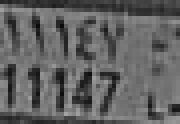
\includegraphics[width=0.3\linewidth]{../assets/plate_gray.png}\quad
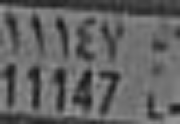
\includegraphics[width=0.3\linewidth]{../assets/plate_box.png}\quad
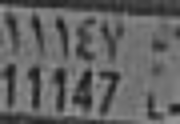
\includegraphics[width=0.3\linewidth]{../assets/plate_gauss.png}\\[2pt]
{\small چپ: اصلی — وسط: جعبه‌ای $5\times5$ — راست: گاوسی $\sigma=1.5$}
\end{center}

جعبه‌ای به‌طورِ یکسان میانگین می‌گیرد (مصنوعاتِ مربعی)؛ گاوسی به مرکز وزنِ بیشتری می‌دهد
(نرم‌تر، طبیعی‌تر).

\begin{riyazi}
کرنلِ گاوسی: $h(i,j) = \dfrac{1}{2\pi\sigma^2}\,e^{-(i^2+j^2)/(2\sigma^2)}$
\newline
$\sigma$ میزانِ تاری را کنترل می‌کند؛ بزرگ‌تر = هموارسازیِ بیشتر و کرنلِ پهن‌تر.
\end{riyazi}

گاوسی \textbf{تفکیک‌پذیر} (\lr{separable}) است: یک گاوسیِ دوبعدی = یک تاریِ افقیِ یک‌بعدی سپس یک
تاریِ عمودیِ یک‌بعدی $\rightarrow$ بسیار سریع‌تر.

\subsection{چرا اصلاً هموار کنیم؟}

\begin{itemize}
  \item حذفِ نویز پیش از آستانه/لبه (نویز لبه‌های کاذب می‌سازد — جلسهٔ ۵).
  \item تاری \emph{پیش} از کاهشِ اندازه برای پرهیز از آلیاسینگ (نایکوئیستِ جلسهٔ ۱).
  \item سرکوبِ بافتِ ریز تا ساختارهای بزرگ غالب شوند (یافتنِ صفحه، نه دانه‌بندیِ کاغذ).
\end{itemize}

\begin{hoshdar}
اما تاری جزئیات را هم نابود می‌کند. زیادی‌اش، ارقام را به هم می‌مالد — یک مبادله که باید تنظیمش کنید.
\end{hoshdar}

% ===================================================================
\section{تیزسازی (Sharpening)}

\textbf{ماسکِ ناتیز} (\lr{unsharp mask}): $\text{تیز} = \text{تصویر} + \lambda(\text{تصویر} -
\text{تار})$. جملهٔ $(\text{تصویر}-\text{تار})$ \emph{همان} جزئیاتِ فرکانس‌بالاست؛ آن را
بازمی‌گرداند تا لبه‌ها (ضربه‌قلم‌های ارقام) برجسته شوند.

\begin{center}
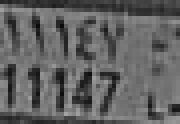
\includegraphics[width=0.42\linewidth]{../assets/plate_gray.png}\quad

\includegraphics[width=0.42\linewidth]{../assets/plate_sharp.png}\\[2pt]
{\small قبل (چپ) و بعد از تیزسازی با ماسکِ ناتیز (راست)}
\end{center}

\begin{hoshdar}
تیزسازی \emph{همه‌چیزِ} فرکانس‌بالا را تقویت می‌کند — از جمله نویز و بلوک‌های JPEG. تیزسازیِ
بیش‌ازحد \textbf{هاله} (حلقه‌های روشن/تاریک) دورِ لبه‌ها می‌سازد. اول نویز را حذف کنید، بعد ملایم
تیز کنید. هرگز یک تصویرِ نویزی را کورکورانه تیز نکنید.
\end{hoshdar}

% ===================================================================
\section{تمرینِ کلاسیِ وسط‌جلسه (۱۲ دقیقه)}

\begin{tamrin}
یک وصلهٔ $3\times3$ و یک کرنل:
\[
P=\begin{bmatrix}10&10&10\\10&50&10\\10&10&10\end{bmatrix}\qquad
K=\begin{bmatrix}0&-1&0\\-1&5&-1\\0&-1&0\end{bmatrix}
\]
(۱) خروجیِ پیکسلِ مرکزی را حساب کنید (ضربِ عنصربه‌عنصر، سپس جمع). (۲) این کرنل با مقدارِ مرکزی چه
می‌کند؟ چه نوع فیلتری است؟ (۳) حالا کرنلِ تاریِ جعبه‌ای را به‌جایش بگذارید. خروجیِ مرکز چیست؟
\end{tamrin}

\textbf{جمع‌بندی:} تیزسازی: $5(50) - 10 - 10 - 10 - 10 = 250 - 40 = 210$. مرکز (۵۰) به ۲۱۰ پرید —
\emph{کنتراست تقویت شد}. این یک فیلترِ \textbf{بالاگذر} است: تفاوتِ مرکز و اطراف را برجسته می‌کند.
تاریِ جعبه‌ای: $(10{\cdot}8 + 50)/9 = 130/9 \approx 14$. مرکزِ روشن \emph{میانگین‌گیری و پایین}
آمد — هموار شد. همان وصله، دو کرنل، دو اثرِ متضاد. کرنل همه‌چیز است.

% ===================================================================
\section{کاربردهای فیلترِ مکانی}

فیلترهای مکانی در تقریباً هر خطِ لولهٔ بینایی‌اند:

\begin{itemize}
  \item \textbf{پیش‌پردازش}: هموارسازیِ ملایم پیش از لبه/آستانه تا نویز، لبه‌های کاذب نسازد.
  \item \textbf{کاهشِ نویز}: گاوسی برای نویزِ گاوسی، میانه برای نمک‌وفلفل، دوطرفه برای حفظِ لبه.
  \item \textbf{تشخیصِ ویژگی}: کرنل‌های گرادیان لبه‌ها را می‌یابند (جلسهٔ ۵)؛ کرنل‌های خاص گوشه و لکه.
  \item \textbf{بهبود}: تیزسازی برای وضوحِ بیشتر (با احتیاط).
  \item \textbf{یادگیریِ عمیق}: لایه‌های اولِ CNN فیلترهای لبه/بافت را \emph{می‌آموزند}.
\end{itemize}

\begin{yaddasht}
یک بینشِ مهم: بیشترِ سیستم‌های بینایی، \emph{زنجیره‌ای} از فیلترهای مکانی‌اند. کیفیتِ نهایی به
انتخابِ درستِ فیلترها و ترتیبشان بستگی دارد. یک فیلترِ غلط در ابتدا (مثلِ تاریِ بیش‌ازحد)،
اطلاعاتی را نابود می‌کند که هیچ گامِ بعدی نمی‌تواند بازگرداند.
\end{yaddasht}

\subsection{جدولِ انتخابِ فیلتر}

\begin{center}
\begin{tabular}{>{\raggedright\arraybackslash}p{0.4\linewidth} >{\raggedright\arraybackslash}p{0.5\linewidth}}
\toprule
\textbf{هدف} & \textbf{فیلترِ پیشنهادی} \\
\midrule
حذفِ نویزِ عمومی، حفظِ کلی & گاوسی \\
حذفِ نویزِ نمک‌وفلفل & میانه \\
هموارسازی با حفظِ لبه & دوطرفه \\
برجسته‌کردنِ لبه‌ها & تیزسازی / گرادیان \\
آماده‌سازی برای کاهشِ اندازه & گاوسی (ضدِ آلیاسینگ) \\
\bottomrule
\end{tabular}
\end{center}

% ===================================================================
\section{بخشِ عمیق}

\subsection{دیدِ فرکانسی: پایین‌گذر در برابرِ بالاگذر}

هموارسازی \textbf{فرکانس‌های پایین} (تغییراتِ آرام) را نگه می‌دارد و بالا را حذف می‌کند (فیلترِ
\textbf{پایین‌گذر}). تیزسازی/لبه \textbf{فرکانس‌های بالا} (تغییراتِ سریع) را نگه می‌دارد — فیلترِ
\textbf{بالاگذر}. جلسهٔ ۶ این را با تبدیلِ فوریه صریح می‌کند؛ امروز شهود است. «تاری = پایین‌گذر،
لبه = بالاگذر» عدسی‌ای است که تا آخرِ کورس استفاده می‌کنید.

\subsection{تصویرِ انتگرالی: تاریِ جعبه‌ای در زمانِ ثابت}

یک ترفندِ زیبا: با یک \textbf{تصویرِ انتگرالی} (\lr{integral image}، که هر پیکسلش مجموعِ همهٔ
پیکسل‌های بالا-چپش است)، می‌توان مجموعِ هر مستطیل را با فقط \emph{چهار} دسترسی حساب کرد — مستقل
از اندازهٔ مستطیل. پس یک تاریِ جعبه‌ای با هر اندازه‌ای در زمانِ ثابت به‌ازای هر پیکسل اجرا می‌شود.
این پشتِ بسیاری از الگوریتم‌های سریعِ کلاسیک (مثلِ تشخیصِ چهرهٔ \lr{Viola-Jones}) است.

\begin{yaddasht}
درسِ کلی: اغلب یک بازنماییِ هوشمندانه (مثلِ تصویرِ انتگرالی) یا یک ویژگیِ ریاضی (مثلِ
تفکیک‌پذیری) می‌تواند یک عملیاتِ به‌ظاهر گران را ارزان کند. این تفاوتِ یک پیاده‌سازیِ سادهٔ کند و
یک سیستمِ بلادرنگ است.
\end{yaddasht}

\subsection{اثراتِ مرزی با جزئیات}

روش‌های مختلفِ پُرکردنِ مرز نتایجِ متفاوت می‌دهند: \lr{zero} (صفر) یک حاشیهٔ تیره می‌سازد؛
\lr{replicate} آخرین پیکسل را تکرار می‌کند؛ \lr{reflect} تصویر را آینه می‌کند (معمولاً طبیعی‌ترین).
برای تصاویرِ کوچک (مثلِ کراپِ کنتور)، اثرِ مرز نسبتاً بزرگ است، پس انتخابِ روشِ درست مهم‌تر می‌شود.

\subsection{تفکیک‌پذیری و سرعت}

یک کرنلِ دوبعدیِ تفکیک‌پذیر = ضربِ بیرونیِ دو کرنلِ یک‌بعدی؛ آن‌ها را پشتِ‌سرِ‌هم اعمال کنید. یک
تاریِ $k\times k$ به‌ازای هر پیکسل $k^2$ ضرب می‌خواهد؛ تفکیک‌شده، فقط $2k$ — بردی بزرگ برای $k$های
بزرگ. OpenCV این را برای گاوسی خودکار انجام می‌دهد؛ بدانیدش تا فیلترهای سریع بنویسید.

\subsection{فیلترِ غیرخطی: میانه (Median)}

\begin{center}
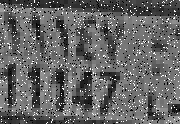
\includegraphics[width=0.42\linewidth]{../assets/plate_noisy.png}\quad
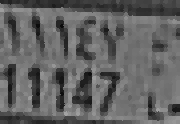
\includegraphics[width=0.42\linewidth]{../assets/plate_median.png}\\[2pt]
{\small نویزِ نمک‌وفلفل (چپ) و میانهٔ $3\times3$ (راست)}
\end{center}

یک فیلترِ \textbf{میانه} میانهٔ همسایگی را می‌گیرد — نه جمعِ وزن‌دار. نویزِ نمک‌وفلفل را می‌کشد
در حالی که لبه‌ها را تیز نگه می‌دارد (گاوسی آن‌ها را می‌مالید). غیرخطی است $\rightarrow$ کانولوشن
نیست، اما همان ایدهٔ «پنجره را بلغزان». داستانِ کاملش در جلسهٔ ۴.

\subsection{فیلترِ خطی در برابرِ غیرخطی}

یک تمایزِ بنیادی: فیلترهای \textbf{خطی} (تاریِ جعبه‌ای، گاوسی، تیزسازی) با یک جمعِ وزن‌دار
کار می‌کنند و همان کانولوشن‌اند؛ خاصیت‌های ریاضیِ خوبی دارند (مثلِ تفکیک‌پذیری). فیلترهای
\textbf{غیرخطی} (میانه، دوطرفه، بیشینه/کمینه) یک تابعِ غیرخطی روی همسایگی اعمال می‌کنند و
کانولوشن نیستند — اما اغلب برای مسائلِ خاص (نویزِ ضربه‌ای، حفظِ لبه) بهترند.

\begin{center}
\begin{tabular}{>{\raggedright\arraybackslash}p{0.28\linewidth} >{\raggedright\arraybackslash}p{0.62\linewidth}}
\toprule
\textbf{ویژگی} & \textbf{خطی / غیرخطی} \\
\midrule
جمعِ وزن‌دار & خطی (کانولوشن) \\
میانه/بیشینه & غیرخطی \\
تفکیک‌پذیری & فقط خطی‌ها \\
حفظِ لبه & میانه، دوطرفه (غیرخطی) بهتر \\
\bottomrule
\end{tabular}
\end{center}

\subsection{فیلترِ دوطرفه (Bilateral)}

تاریِ گاوسی لبه‌ها را می‌مالد؛ فیلترِ \textbf{دوطرفه} با \emph{هم} فاصله \emph{و} شباهتِ شدت
وزن می‌دهد. نتیجه: نواحیِ تخت هموار می‌شوند، لبه‌ها تیز می‌مانند — عالی پیش از آستانه‌گذاریِ یک
سند. کندتر، اما اغلب هموارسازِ درست برای DocScan: \lr{cv2.bilateralFilter}.

% ===================================================================
\section{فیلترها در کد}

\begin{ltrcode}
\begin{lstlisting}[language=Python]
box    = cv2.blur(img, (5, 5))
gauss  = cv2.GaussianBlur(img, (7, 7), 1.5)
median = cv2.medianBlur(img, 3)
k = np.array([[0,-1,0],[-1,5,-1],[0,-1,0]])
sharp  = cv2.filter2D(img, -1, k)          # apply any custom kernel
\end{lstlisting}
\end{ltrcode}

\lr{cv2.filter2D} با هر کرنلی که بدهید کانولوشن می‌کند — ابزارِ عمومی. برای فهمِ عمیق، یک‌بار
کانولوشن را از صفر با \lr{NumPy} پیاده کنید:

\begin{ltrcode}
\begin{lstlisting}[language=Python]
def convolve3x3(img, k):
    h, w = img.shape
    pad = np.pad(img.astype(np.float32), 1, mode='reflect')  # handle borders
    out = np.zeros_like(img, dtype=np.float32)
    for y in range(h):
        for x in range(w):
            region = pad[y:y+3, x:x+3]
            out[y, x] = np.sum(region * k)          # multiply + sum
    return np.clip(out, 0, 255).astype(np.uint8)
\end{lstlisting}
\end{ltrcode}

این نسخهٔ آموزشی (با حلقه) کند است اما مفهوم را روشن می‌کند. در عمل \lr{cv2.filter2D} همین را
هزاران برابر سریع‌تر (برداری‌شده و بهینه) انجام می‌دهد. نکته: با \lr{np.pad} مرزها را مدیریت
کردیم و به یک بافرِ خروجیِ جدا نوشتیم.

\subsection{پارامترها و دام‌ها}

\begin{itemize}
  \item \textbf{اندازهٔ کرنل}: باید فرد باشد ($3, 5, 7, \dots$) تا مرکزِ مشخص داشته باشد.
  \item \textbf{$\sigma$ گاوسی}: اگر ۰ بدهید، OpenCV از اندازهٔ کرنل محاسبه‌اش می‌کند؛ برعکس هم.
  \item \textbf{عمقِ خروجی}: \lr{filter2D} با \lr{-1} همان نوعِ ورودی؛ اما کرنل‌های لبه مقادیرِ منفی می‌دهند که در \lr{uint8} بریده می‌شوند — به \lr{float} بروید.
  \item \textbf{مرز}: پیش‌فرضِ \lr{reflect} معمولاً بهتر از \lr{zero} است (لبه‌های تیرهٔ مصنوعی نمی‌سازد).
\end{itemize}

\begin{hoshdar}
دامِ رایج: اعمالِ یک کرنلِ لبه (با مقادیرِ منفی) روی تصویرِ \lr{uint8} — نتایجِ منفی به صفر بریده
می‌شوند و نیمی از لبه‌ها ناپدید می‌شوند. برای فیلترهایی که خروجیِ منفی دارند، ابتدا به
\lr{float32} تبدیل کنید و در آخر نرمال‌سازی/قدرمطلق بگیرید.
\end{hoshdar}

% ===================================================================
\section{باغِ کرنل‌ها و طراحیِ آن‌ها}

شما کرنل‌ها را حفظ نمی‌کنید — می‌فهمید «میانگین» در برابرِ «تفاضل» چه می‌کند و بقیه را طراحی
می‌کنید:

\begin{center}
\begin{tabular}{>{\raggedright\arraybackslash}p{0.35\linewidth} >{\raggedright\arraybackslash}p{0.55\linewidth}}
\toprule
\textbf{کرنل} & \textbf{اثر} \\
\midrule
همه $1/n$ & تاریِ جعبه‌ای (میانگین) \\
وزن‌های گاوسی & تاریِ نرم \\
مرکز ۵، اطراف $-1$ & تیزسازی (بالاگذر) \\
سطرهای $[-1,0,1]$ & گرادیانِ افقی (لبه، جلسهٔ ۵) \\
هویت + (هویت $-$ تار) & ماسکِ ناتیز \\
\bottomrule
\end{tabular}
\end{center}

\textbf{منطقِ طراحی:} اگر می‌خواهید هموار کنید، کرنلی بسازید که مجموعِ مثبت داشته و به مرکز وزن
دهد. اگر می‌خواهید تغییرات (لبه) را برجسته کنید، کرنلی با مجموعِ صفر بسازید که تفاوتِ همسایه‌ها را
می‌گیرد. این دو الگو، پشتِ تقریباً همهٔ فیلترهای خطی‌اند.

\begin{yaddasht}
یک کرنلِ جالب: \textbf{برجسته‌سازی} (\lr{emboss}) با $\begin{bmatrix}-2&-1&0\\-1&1&1\\0&1&2\end{bmatrix}$
که یک اثرِ سه‌بعدیِ نور از یک جهت می‌سازد. این نشان می‌دهد چطور چیدمانِ نامتقارنِ اعداد، جهت‌داری
ایجاد می‌کند — همان ایده که در تشخیصِ لبهٔ جهت‌دارِ جلسهٔ ۵ به کار می‌آید.
\end{yaddasht}

% ===================================================================
\section{کانولوشن در برابرِ همبستگی}

یک نکتهٔ نظری که در عمل مهم می‌شود: \textbf{کانولوشن} کرنل را پیش از اعمال ۱۸۰ درجه می‌چرخاند،
اما \textbf{همبستگی} (\lr{correlation}) نه. برای کرنل‌های متقارن (مثلِ گاوسی یا تاریِ جعبه‌ای)
این دو نتیجهٔ یکسان می‌دهند، پس اغلب تفاوتی حس نمی‌کنید. اما برای کرنل‌های نامتقارن (مثلِ تشخیصِ
لبهٔ جهت‌دار)، اهمیت دارد. \lr{cv2.filter2D} در واقع همبستگی انجام می‌دهد؛ اگر کانولوشنِ واقعی
می‌خواهید، کرنل را اول بچرخانید.

\begin{nokte}
در یادگیریِ عمیق، آنچه «لایهٔ کانولوشن» نامیده می‌شود در واقع همبستگی است (کرنل چرخانده نمی‌شود).
چون شبکه کرنل را از داده می‌آموزد، چرخشِ آن اهمیتی ندارد — شبکه هر طور که لازم باشد یاد می‌گیرد.
این یک نمونه از جاهایی است که اصطلاحاتِ ریاضی و عملی کمی متفاوت‌اند.
\end{nokte}

% ===================================================================
\section{این جلسه در پروژهٔ نهایی}

در DocScan، هموارسازی نقشِ حیاتی دارد اما ظریف است: یک تاریِ \emph{ملایم} پیش از آستانه‌گذاری،
نویز را حذف می‌کند و آستانهٔ تمیزتری می‌دهد؛ اما تاریِ \emph{زیاد} ارقام را به هم می‌مالد و
جداسازیِ رقم‌ها (جلسهٔ ۹) را خراب می‌کند. برای عکس‌های موبایلیِ نویزی، فیلترِ دوطرفه یا میانه
اغلب بهترند از گاوسی، چون لبه‌های ارقام را حفظ می‌کنند.

\begin{yaddasht}
یک قاعدهٔ عملی: کوچک‌ترین تاری‌ای را که نویز را کافی حذف کند به کار ببرید. هر واحدِ تاریِ اضافه،
جزئیاتی است که برای خواندنِ رقم از دست می‌دهید. این تعادل را روی چند تصویرِ سخت تنظیم کنید.
\end{yaddasht}

% ===================================================================
\section{جمع‌بندی}

\begin{itemize}
  \item توضیحِ کانولوشن و اینکه چطور یک کرنل عملیات را تعریف می‌کند.
  \item هموارسازی با جعبه/گاوسی؛ تیزسازی با ماسکِ ناتیز؛ دانستنِ مبادله‌ها.
  \item مدیریتِ مرز و نرمال‌سازی؛ بهره‌گیری از تفکیک‌پذیری برای سرعت.
  \item دیدِ پایین‌گذر/بالاگذر و پیوند به CNNها.
\end{itemize}

\begin{tamrin}
\textbf{تحویلیِ این هفته (پیش از جلسهٔ ۴):} روی تصاویرِ واقعیِ کنتور/پلاک: (۱) یک کانولوشنِ
$3\times3$ را \emph{از صفر} (\lr{NumPy}) پیاده و با \lr{cv2.filter2D} تطبیق دهید. (۲) تاریِ
جعبه‌ای و گاوسی را در چند اندازه مقایسه کنید؛ از‌دست‌رفتنِ جزئیات در برابرِ حذفِ نویز را بحث کنید.
(۳) یک پلاک را با ماسکِ ناتیز تیز کنید؛ بیابید کجا شروع به ساختنِ هاله می‌کند. (۴) یادداشت: چه
تاری‌ای به آستانهٔ DocScanِ شما کمک می‌کند و چه تاری‌ای ارقام را بیش‌ازحد می‌مالد؟
\end{tamrin}

\subsection*{واژه‌نامهٔ کوتاه}

\begin{center}
\begin{tabular}{>{\raggedright\arraybackslash}p{0.3\linewidth} >{\raggedright\arraybackslash}p{0.6\linewidth}}
\toprule
\textbf{اصطلاح} & \textbf{معنی} \\
\midrule
\lr{Convolution} & لغزاندنِ یک کرنل و جمعِ وزن‌دارِ همسایگی \\
\lr{Kernel / Filter} & ماتریسِ کوچکی که عملیات را تعریف می‌کند \\
\lr{Low-pass / High-pass} & نگه‌داشتنِ فرکانسِ پایین (تاری) / بالا (لبه) \\
\lr{Separable} & کرنلِ دوبعدی = دو کرنلِ یک‌بعدی (سریع‌تر) \\
\lr{Unsharp mask} & تیزسازی با افزودنِ جزئیاتِ فرکانس‌بالا \\
\lr{Median / Bilateral} & فیلترِ غیرخطیِ حفظ‌کنندهٔ لبه \\
\bottomrule
\end{tabular}
\end{center}

\vspace{0.5cm}
\begin{center}
\textit{کرنل، الگوریتم است. تاری، تیزی، لبه — همه یک عملیات با اعدادِ متفاوت.}
\end{center}

\end{document}
